\documentclass[12pt, twoside]{article}
\usepackage{jmlda}
\newcommand{\hdir}{.}
\usepackage[utf8]{inputenc}
\usepackage[english,russian]{babel}
\usepackage{graphicx}
\newcommand{\real}{\mathbb{R}}
\newcommand{\nat}{\mathbb{N}}
\newcommand{\integ}{\mathbb{Z}}
\usepackage{bm}
\usepackage{multicol}
\usepackage{graphicx}
\graphicspath{{img/}}
\DeclareGraphicsExtensions{.pdf,.png,.jpg}
%\usepackage[round]{natbib}
%\usepackage[
%backend=biber,
%style=alphabetic,
%sorting=ynt
%]{biblatex}

%\addbibresource{Kulagin.bib}



\begin{document}

%\nocite{*}

\title
    [Шаблон статьи для публикации] % краткое название; не нужно, если полное название влезает в~колонтитул
    {Построение метода динамического выравнивания многомерных временных рядов, устойчивого к локальным колебаниям сигнала.}
\author
    [И.\,О.~Автор] % список авторов (не более трех) для колонтитула; не нужен, если основной список влезает в колонтитул
    {И.\,О.~Автор, И.\,О.~Соавтор, И.\,О.~Фамилия} % основной список авторов, выводимый в оглавление
    [И.\,О.~Автор$^1$, И.\,О.~Соавтор$^2$, И.\,О.~Фамилия$^{1,2}$] % список авторов, выводимый в заголовок; не нужен, если он не отличается от основного
\email
    {author@site.ru; co-author@site.ru;  co-author@site.ru}
\thanks
    {Работа выполнена при
     %частичной
     финансовой поддержке РФФИ, проекты \No\ \No 00-00-00000 и 00-00-00001.}
\organization
    {$^1$Организация, адрес; $^2$Организация, адрес}
\abstract
    {Данная работа посвящена построению эффективного алгоритма динамического выравнивания многомерных временных рядов. Для решения данной задачи предлагается использовать функцию расстояния DTW между двумя многомерными временными рядами, согласно которому выравниваются две оси времени, при этом внутри функционала DTW выбирается расстояние между i-м и j-м измерениями такое, что оно устойчиво к локальным “сдвигам” сигнала. В качестве решения будет рассмотрено более продвинутое, основанное на DTW между парой измерений. Для проверки корректности используются как и реальные данные, например измерения активность мозга обезьян, так и искусственно сгенерированные, например движение сигнала в пространстве по часовой и против часовой стрелки.
	
\bigskip
\noindent
\textbf{Ключевые слова}: \emph {многомерные временные ряды; DTW; динамическое выравнивание.}
}

\maketitle
\linenumbers

\section{Введение}

В данной работе исследуется проблема динамического выравнивания многомерных временных рядов, устойчивого к локальным колебаниям сигнала.
Временной ряд -  собранный в разные моменты времени статистический материал о значении каких-либо параметров (в простейшем случае одного исследуемого процесса). В данном случае рассматривается многомерный случай.

Необходимость сравнивать 2 временных ряда на схожесть возникает из практических задач таких как классификация геномных сигналов \cite{SalvadorC07} 

При этом необходимо учитывать, что в таких задачах как ... возникает необходимо учитывать, что близость временных рядов не ограничивается сдвигами по времени, а также присутствует  расположениям сигналов.

Для сравнения определения расстояния между временными рядами будет использовать известный алгоритм DTW..., однако возникает проблема определения расстояния между сигналами в этом алгоритме.

Базовое решение задачи с помощью метрики L2 расстояния между рядами не всегда оказывается эффективным. Таким примером являются 2 временных ряда, полученные при близком расположении датчиков с сигналами, которые могут зафиксировать один и тот же пик. Полученный пик окажет большое влияние на значение метрики L2.

Напротив, использование известного алгоритма DTW, но уже в многомерном случае позволит обойти проблему малого расстояния между датчиками, как более частный метод для решения конкретного типа задач.

Итак, в данной работе рассматриваются 2 варианта расстояния между сигналами L2 и DTW, выравнивание по временной оси будет сглаживать DTW.

Полученные алгоритмы тестировались на реальных данных и искуственно сгенерированных. Полученные результаты показали преимущество использования попарного DTW алгоритма.


\section{Постановка задачи.}

Рассматривается алгоритм решения задачи динамического выравнивания многомерных рядов.

Задача классификации временных рядов имеет вид.

Пусть X - множество временных рядов, Y - множество меток классов.

$\forall x \in X x \in \mathbb{R^K}$

При $|Y| = 2$ рассматривается задача бинарной классификации, при $|Y| \geq 2$ - многоклассовой классификации.

Предполагается существование зависимости $f: X \rightarrow Y$

Задача заключается в поиске оптимального алгоритма из семейства $A = \{a_{\alpha}\}$, предсказывающего класс из множества Y.

Пусть $X^n = \{X_1, X_2 \dots X_n\}$ - обучающая выборка из временных рядов, $Y^n = \{Y_1, Y_2 \dots Y_n\}$ - метки классов.

В качестве алгоритмов классификации будем использовать метрические алгоритмы классификации. Поэтому введём функцию расстояния между 2 временными рядами с помощью алгоритма DTW.

$D(i, j) = d(i, j) + min(D(i - 1, j), D(i, j - 1), D(i - 1, j - 1))$

$d(i, j)$ - расстояние между парой сигналов. Определяется 2 разными способами.

1) L2 - метрика.

$d(i, j) = \Sigma_{k = 1}^K(X(i, k) - X(j, k))^2$

2) DTW - расстояние.

$d(i, j, k, t) = (X(i, k) - X(j, t)) ^ 2 + min(d(i, j, k - 1, t), d(i, j, k, t - 1), d(i, j, k - 1, t - 1))$

$d(i, j) := d(i, j, K, K)$

В качестве функционала ошибки будем рассматривать accuracy = $\frac{TP + TN}{TP + TN + FP + FN}$

Будут рассматриваться искусственно сгенерированные данные, которые жестко будут разделены по положению пика на 2 класса.

Те ряды, которые имеют небольшое расстояние до пика, будут принадлежать одному классу.

А также многомерные сигналы, которые которые замерялись на поверхности мозга обезьян. Датчики при этом находились на небольшом расстояниии друг от друга. 


\section{Вычислительный эксперимент}

\subsection{Цель эксперимента}

Данный эксперимент проводится для того, чтобы обнаружить примеры, когда алгоритм, устойчивый к локальным отклонениям сигнала

показывает лучшую точность в задаче классификации. Для этого будут сравниваться реальные данные и искусственные.

Также немаловажную роль будет играть время работы алгоритма, так как способ с DTW расстоянием медленнее.

\subsection{Ход эксперимента}

Эксперимент проводится в 2 этапа.

1.\textbf{Искусственно сгенерированные данные}, на которых можно увидеть достоинства и недостатки работы алгоритмов и предложить из улучшение.

2.\textbf{Реальные данные}, на которых можно протестировать полученные алгоритмы и измерить качество.

3. Временной эксперимент оценит время работы каждого из алгоритмов.

Генерация многомерных временных рядов из 1 шага использовался шаблон 2 измерений.

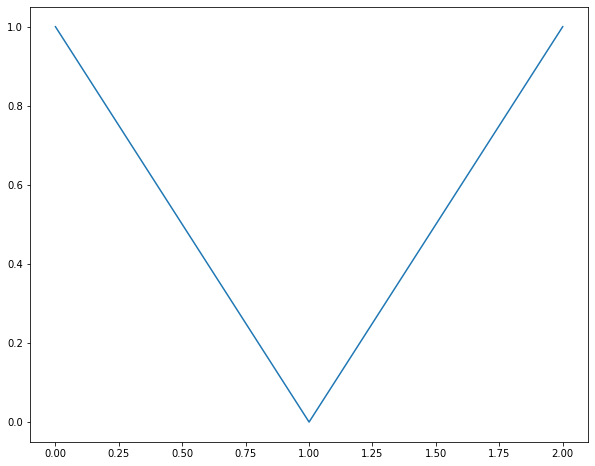
\includegraphics[width=3cm, height=4cm]{sample1}


Данные были получены генерацией 3 перемещающихся шаблонов типа 1, а остальные значения временного ряда были заполнены шаблоном типа 2.

При этом если обозначить общее количество данных как $4k$, то количество данных, в которых шаблон 1 находится слева будет равняться

$k$, шаблон справа - тоже.



Суть 2 этапа заключается в проверке полученных на 1 шаге алгоритмов на реальных данных и измерением точности.

В итоге будет выбран лучший алгоритм.

К сожалению, обыкновенный L2 классифицировал ряды ненамного хуже по метрике accuracy временные ряды.


Этап 3 показал, что DTW внутри DTW работает гораздо медленнее, чем DTW c расстоянием L2 внутри сигналов.


\section{Заключение}

В результате исследования алгоритмов DTW c метриками расстояния между сигналами DTW и L2 было обнаружено, что первый из алгоритмов классифицирует лучше на некотором специфическом наборе данных. Однако время его работы оставляет желать лучшего, значит следует использовать
только в особых случаях.


\nocite{*}
 
\bibliographystyle{unsrt}
\bibliography{Kulagin}

\end{document}